\documentclass[a4paper,french, titlepage]{book}

\usepackage[utf8]{inputenc}   % accents
\usepackage[T1]{fontenc}      % caractères français
\usepackage[french]{babel}    % langue
\usepackage[top=20mm, bottom=20mm, left=20mm , right=20mm]{geometry}		  % package marges
\usepackage{graphicx}         % images
\usepackage[graphicx]{realboxes}
\usepackage{verbatim}         % texte préformaté
\usepackage{moreverb}
\usepackage{amsmath,amsfonts,amssymb,amsthm}
\usepackage[all]{xy}		  % diagrammes
\usepackage{float} 			  % images
\usepackage{lscape}			  % pages paysage
\usepackage{url}			  % bibliographie
\usepackage{xcolor}			  % couleurs
\usepackage{verbatim, textcomp, fancyvrb,multicol} % programmes
\usepackage{framed}								   % programmes je crois
\usepackage{listings} % code java en couleurs
\usepackage{subfig}
%\usepackage{subfigure}
\usepackage{wrapfig}
\usepackage{mathrsfs}
\usepackage{amsmath}
\usepackage{hyperref}
\hypersetup{
    colorlinks = true,
    allcolors = {black}
}




% Personnalisation entêtes et pieds de pages
%\usepackage{mathpazo} % nouvelle police 
%\usepackage{fancyhdr}
%\pagestyle{fancy}

% Entêtes
%\renewcommand{\headrulewidth}{1pt}
%\fancyhead[C]{} 
%\fancyhead[L]{TER}
%\fancyhead[R]{Commande d'une ligne transitique MONTRAC}
%\headheight=1.1cm

% Pieds de pages
%\renewcommand{\footrulewidth}{1pt}
%\fancyfoot[C]{Bruno \bsc{Dato}, Abdellah \bsc{Elgourain} et Evgeny \bsc{Shulga}} 
%\fancyfoot[L]{M1 EEA / ISTR}
%\fancyfoot[R]{\thepage}

\title{{\Huge STAGE}\\Intégration et commande sous ROS du robot Baxter au sein d'une cellule flexible d'assemblage\\}
\author{Bruno \bsc{Dato}}
\date{30 juin 2016}


\begin{document}
 
%\maketitle  %page de garde
\thispagestyle{empty}

\begin{center}
Master 1 Électronique Électrotechnique Automatique, Ingénierie des Systèmes Temps-Réel  
\vspace{0.5cm}

\begin{figure}[H] 
\begin{center}

\includegraphics[scale=0.3]{Images/logo_ups.jpg} 
\end{center}
\end{figure}





\vspace{0.3cm}

{\Huge STAGE}\\

\vspace{0.3cm}

{\Huge Intégration et commande sous ROS du robot Baxter au sein d'une cellule flexible d'assemblage}\\

\vspace{0.5cm}

\begin{figure}[H] 
\begin{center}
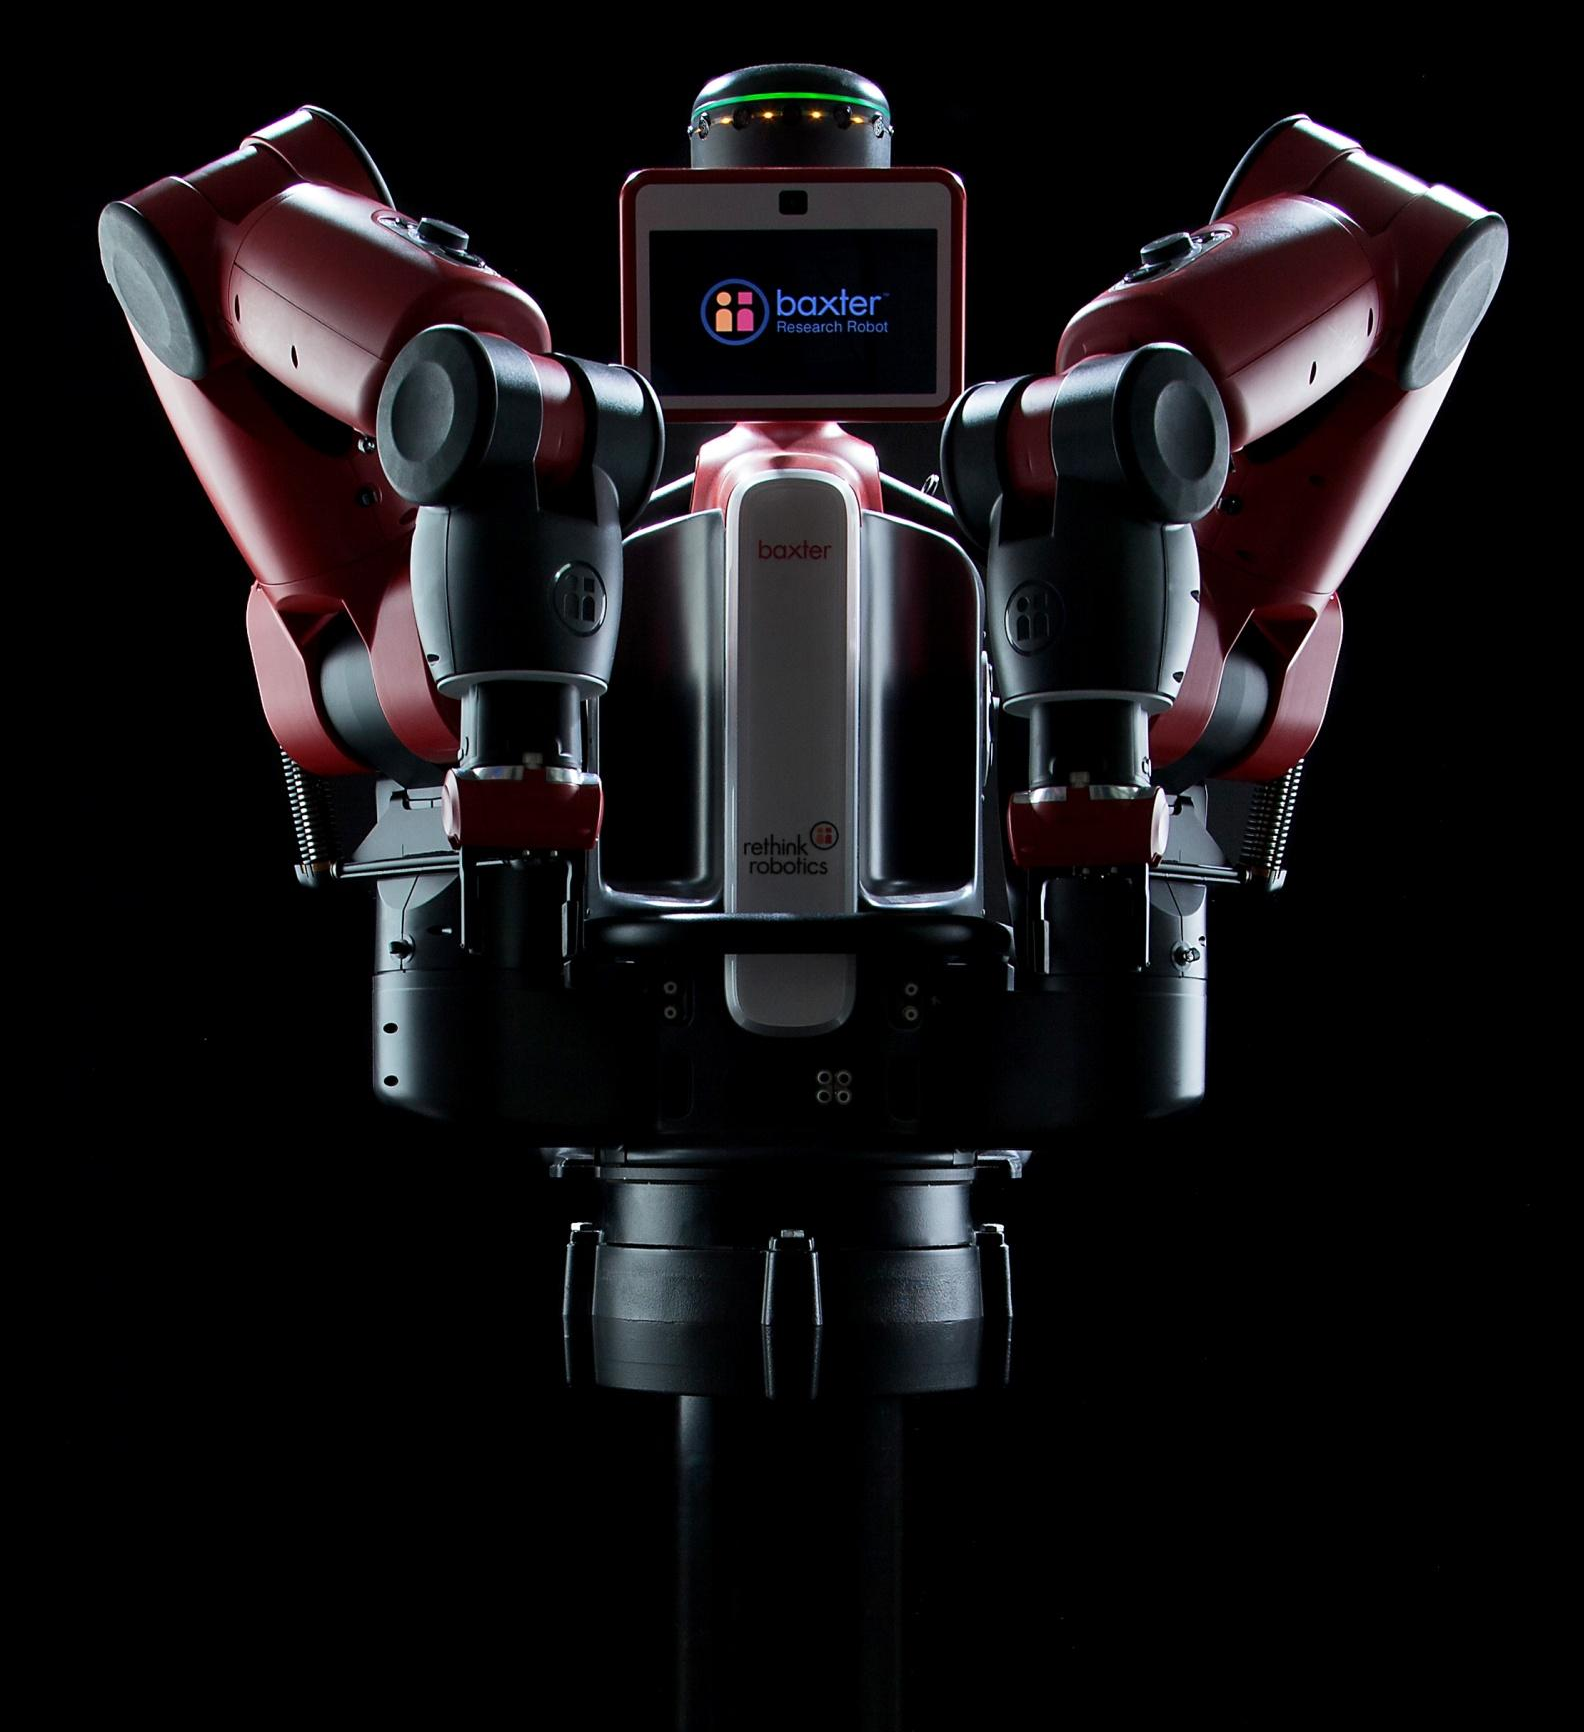
\includegraphics[scale=0.2]{Images/baxter.png}
\end{center}
\end{figure}

\vspace{0.5cm}

{\LARGE Auteur}\\

\vspace{0.2cm}

Bruno \bsc{Dato}\\

\vspace{0.5cm}

{\Large Encadrants}\\

\vspace{0.2cm}

C. Briand, M. Taïx\\ 



\vspace{1cm}


30 juin 2016




\end{center}

\newpage
\addcontentsline{toc}{section}{Remerciements}
\chapter*{Remerciements}

\vspace{5cm}

Je tiens à remercier mes encadrant de stage C. Briand et M. Taïx pour m'avoir permis de réaliser ce stage. Je remercie aussi toutes les personnes de l'AIP pour leur accueil au sein de la halle technologique durant toute la durée de mon stage.

\newpage
\renewcommand{\contentsname}{Sommaire} % permet de changer le titre de la table des matières
\tableofcontents %sommaire


\newpage
\addcontentsline{toc}{section}{Introduction}
\chapter*{Introduction}


\newpage
\chapter{Présentation du stage}

\section{Projet global}

\vspace{1cm}

Mon stage s'est déroulé au pôle AIP/PRIMECA, à Toulouse, sur le campus de l'université Paul Sabatier à la halle technologique. Ces locaux disposent de divers systèmes tels que des robots mobiles, des robots manipulateurs, une cellule flexible de production, un vidéo projecteur interactif, un réseau de caméras... Dans le cadre de mon stage, j'ai travaillé sur l'interaction entre un des robot manipulateurs : le robot Baxter, et la ligne transitique MONTRAC sur laquelle j'avais déjà effectué mon projet de TER.\\

\vspace{1cm}

Ce stage s'inscrit dans un projet de plus grande envergure visant à faire interagir de nombreux systèmes se trouvant à la halle technologique comme vous pouvez le voir sur la figure \ref{projet_global}. En effet, depuis 2 ans, il y a eu différents projets et stages concernant le vidéo projecteur interactif, la ligne transitique et le réseau caméras. 

\vspace{1cm}

\begin{figure}[H] 
\begin{center}
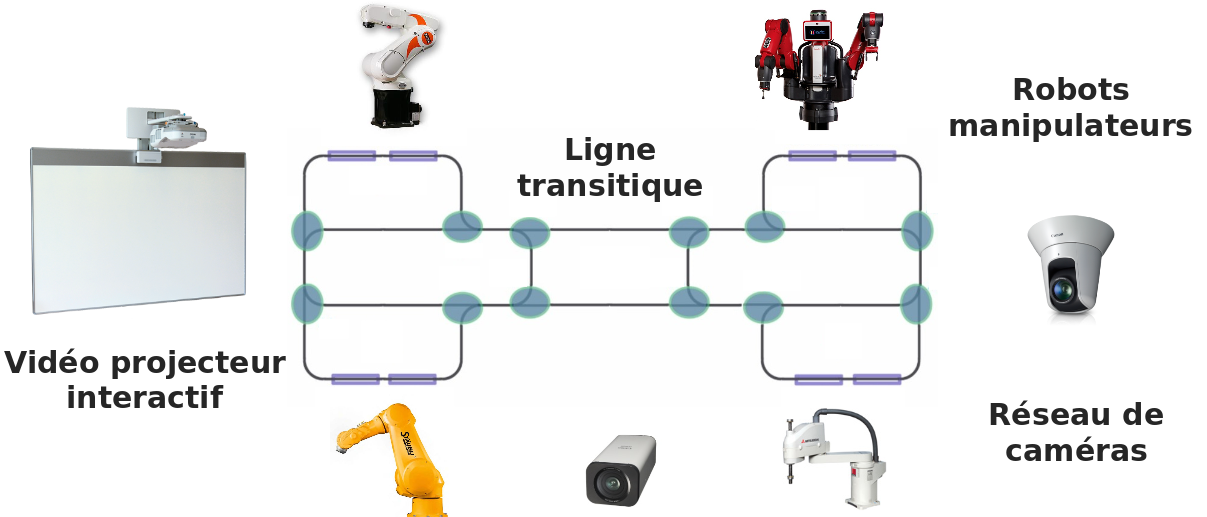
\includegraphics[scale=0.35]{Images/projet_global.png} 
\end{center}
\caption{Vue globale des systèmes à faire interagir dans un futur proche}
\label{projet_global}
\end{figure} 

\vspace{1cm}

\newpage
\section{Le robot Baxter \label{section_lerobotbaxter}}

\begin{wrapfigure}[15]{r}{6cm}
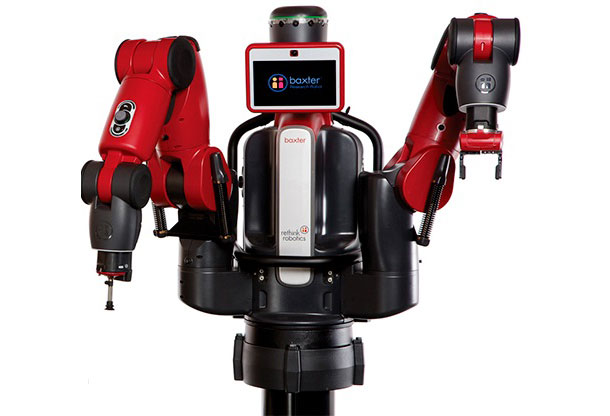
\includegraphics[scale=0.3]{Images/baxter_hum.jpg}
\caption{Le robot collaboratif Baxter}
\label{baxter_hum}
\end{wrapfigure}

Le robot Baxter est un robot humanoïde collaboratif plus communément appelé cobot. Il a été conçu par Rodney Brooks et sa société Rethink Robotics. Un des principaux atouts de ce robot est que sa version dédiée à la recherche peut être commandé à l'aide du middleware ROS qui est très utilisé aujourd'hui en robotique.\\

Baxter dispose de deux bras manipulateurs comme vous pouvez le voir sur la figure \ref{baxter_hum}, chacun de ces deux bras peut être équipé de pinces ou de ventouses reliés à un système pneumatique. Il dispose de différents capteurs : un accéléromètre, un capteur infrarouge et une caméra sur chaque bras. Il possède aussi une troisième caméra et un sonar au niveau de sa tête, le sonar lui permet de détecter en 3D des objets ou des humains lorsqu'ils sont à une certaine distance. Il possède aussi différents boutons sur ces bras et ses épaules qui permettent d'interagir directement avec lui à l'aide de l'écran situé sur sa tête. Enfin il est possible de déplacer ses bras en les saisissant par leur manchette (chaque manchette est munie d'un capteur de pression).\\

Durant mon stage, j'ai surtout travaillé sur le mouvement des bras manipulateurs équipés de pinces afin de saisir et poser des objets bien qu'ils soient hypothétiques. Chaque bras possède sept degrés de liberté qui sont les angles de rotation \emph{S1}, \emph{E0}, \emph{E1}, \emph{W0}, \emph{W1} et \emph{W2} que vous pouvez voir sur la figure \ref{Baxter_arm} ci dessous.



\begin{figure}[H] 
\begin{center}
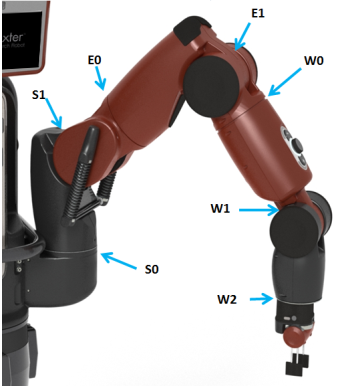
\includegraphics[scale=0.7]{Images/Baxter_arm.png} 
\end{center}
\caption{Les différents angles des bras du robot Baxter}
\label{Baxter_arm}
\end{figure} 

Pour le mouvement des bras, Baxter dispose de quatre modes différents :

\begin{itemize}
\item[ ]
\item[•] \textbf{Joint Position Control} : Il faut spécifier les valeurs de position que l'on souhaite atteindre pour chacun des sept angles. Le mouvement est ensuite contrôlé automatiquement par Baxter afin d'éviter des collisions entre les deux bras ou avec Baxter lui même mais aussi des positions impossibles. La vitesse est aussi contrôlée.
\item[•] \textbf{Raw Joint Position Control} : C'est le même fonctionnement que le mode Joint Position Control cependant, le mouvement est moins contrôlé cette fois : il n'y a plus d'évitement des collisions et les bras se déplacent à la vitesse maximale que Baxter peut fournir. Il faut donc faire très attention avec ce mode.
\item[•] \textbf{Joint Velocity Control} : Il faut spécifier les valeurs de vitesse que l'on souhaite atteindre pour chacun des sept angles. Il y a à nouveau un contrôle pour éviter les collisions cependant la vitesse maximale peut être atteinte.
\item[•] \textbf{Joint Velocity Control} : Il faut spécifier les valeurs de moment (ou couple) que l'on souhaite atteindre pour chacun des sept angles. Pour ce mode, les contrôles du mouvement sont minimes, il faut donc l'utiliser avec beaucoup de précautions.
\item[ ]
\end{itemize}

Pour les commandes que nous verrons par la suite, j'ai utilisé le premier mode : Joint Position Control, couplé avec un service ROS proposé par le robot. Le service permet, à partir d'une position cartésienne dans l'espace ainsi que d'une orientation souhaitée pour l'extrémité d'un des bras, de fournir les valeurs de position des sept angles qui permettent d'atteindre cette disposition.

\section{Ligne transitique MONTRAC$^{\circledR}$}

\subsection{Présentation}

La ligne transitique MONTRAC est composée de rails alimentés en énergie électrique sur lesquels circulent des navettes. Les navettes ne peuvent se déplacer que dans un sens sur ces rails.\\
     
Pour commander la ligne, on dispose de cinq automates programmables industriels que nous appellerons API. Il y en a 2 de la marque Siemens$^{\circledR}$ et 3 de type Schneider$^{\circledR}$. Ces automates gèrent les différents actionneurs et capteurs situés sur les rails. Les navettes ne sont pas programmables, une fois allumées elles avancent jusqu'à ce qu'on les arrête. Elles possèdent un capteur de proximité situé à l'avant pour éviter les collisions entre les navettes et les stopper lorsqu'elles rencontrent un obstacle.\\       

Cette ligne comporte 5 "secteurs" dont un central et 4 postes de travail. Chaque "secteur" est contrôlé par un des API qui agit sur la ligne via un système d'air comprimé. Les zones 1 à 3 correspondent aux automates Schneider$^{\circledR}$ et les deux autres zones correspondent aux automates Siemens$^{\circledR}$. La ligne possède 12 aiguillages comme on peut le voir sur la figure \ref{Les zones de travail}.

\begin{figure}[H] 
\begin{center}
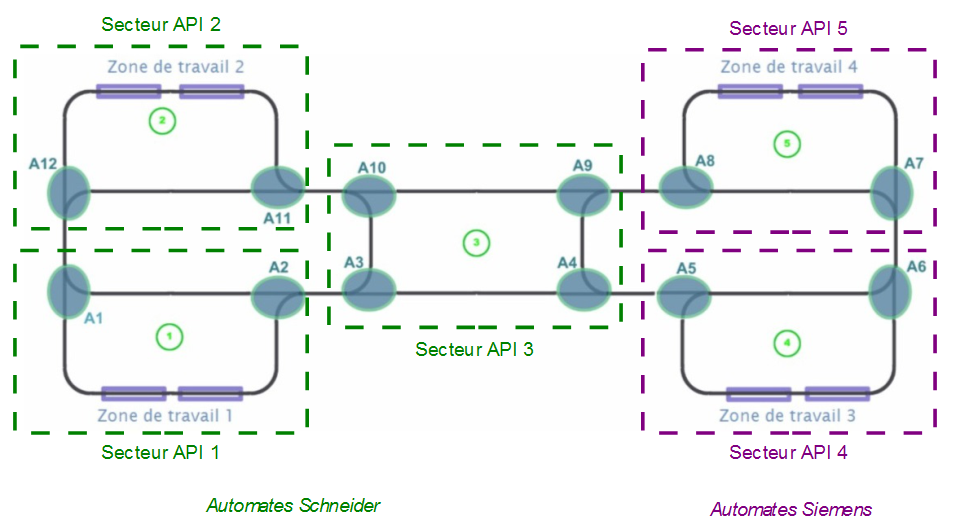
\includegraphics[scale=0.65]{Images/zone_travail.png} 
\end{center}
\caption{Schéma simplifié de la ligne transitique}
\label{Les zones de travail}
\end{figure} 


\newpage
\subsection{Capteurs et actionneurs}

Les actionneurs permettent de commander les points d'arrêts des navettes, les aiguillages et des ergots pouvant bloquer les navettes à certains endroits lorsqu'elles sont arrêtées. Les capteurs nous permettent de connaître les positions des navettes, des aiguillages et des ergots. Les listes des actionneurs et capteurs sont données ci-dessous.

\begin{table}[H]

 
\begin{center}
\begin{tabular}{|c||l|}
	\hline RxG   & Positionne l'aiguillage x à gauche  \\
	\hline RxD   & Positionne l'aiguillage x à droite  \\
	\hline Dx    & Dévérrouille l'aiguillage X          \\
	\hline Vx    & vérrouille l'aiguillage X            \\
	\hline STx   & Quand STx vaut 0, les navettes s'arrêtent au niveau de l'actionneur \\
	\hline PIx    & Blocage des navettes sur le poste de travail \\
	\hline
\end{tabular}     
\end{center}
\caption{\label{tab:actionneurs}Actionneurs}
\end{table}
\

\begin{table}[H]

 	  
\begin{center}
	\begin{tabular}{|c||l|}
	\hline CPx   & Capteur de Position. Vaut 1 quand une navette est sur le capteur \\
	\hline PSx   & Capteur de Stop situé juste en face d'un actionneur STx pouvant arrêter la navette \\
	\hline CPIx  & Vaut 1 quand l'ergot PI est sorti      \\
	\hline DxD   & Vaut 1 quand l'aiguillage x est à droite         \\
	\hline DxG   & Vaut 1 quand l'aiguillage x est à gauche \\
	\hline
	\end{tabular}        
\end{center}
\caption{\label{tab:capteurs}Capteurs}
\end{table}

Durant ce stage, j'ai commandé de la ligne via les API des zones 1 et 2 (automates Schneider$^{\circledR}$). Ces automates disposent de 16 entrées et sorties chacun mais toutes ne sont pas utilisées. Les tables \ref{tab:ap1} et \ref{tab:ap2} décrivent respectivement le câblage des API 1 et 2. \\

On peut voir sur la figure~\ref{Schema_detaille} une vision globale de la ligne transitique avec tous les capteurs et actionneurs, les zones contrôlées par les API ainsi que les orientations de chaque rail.

\newpage
\begin{center}
\Rotatebox{90}{%
\begin{minipage}{1.5\linewidth}
\begin{table}[H]
	\begin{center}
		\begin{tabular}{|c|c|c|c|c|c|c|c|c|c|c|c|c|c|c|c|c|c|c|c|c|c|c|c|}
			\hline \multicolumn{2}{|c|}{\textbf{OUT}}  & \multicolumn{2}{|c|}{A1} & \multicolumn{2}{|c|}{V1} & \multicolumn{2}{|c|}{A2} & \multicolumn{2}{|c|}{V2} & \multicolumn{2}{|c|}{S1} & \multicolumn{2}{|c|}{S2} & \multicolumn{2}{|c|}{S3} & \multicolumn{2}{|c|}{S4} & \multicolumn{2}{|c|}{S5} & \multicolumn{2}{|c|}{UP1} & \multicolumn{2}{|c|}{UP2}  \\
			\hline \multicolumn{2}{|c|}{} & R1D & R1G & V1 & D1 & R2D & R2G & V2 & D2 & \multicolumn{2}{|c|}{ST1} & \multicolumn{2}{|c|}{ST2} & \multicolumn{2}{|c|}{ST3} & \multicolumn{2}{|c|}{ST5} & \multicolumn{2}{|c|}{ST4} & \multicolumn{2}{|c|}{PI1} & \multicolumn{2}{|c|}{PI2} \\
			\hline \multicolumn{2}{|c|}{\textbf{IN}} & 0 & 1 & 2 & 3 & 4 & 5 & 6 & 7 & 8 & 9 & 10 & 11 & 12 & 13 & 14 & 15 & & & & & & \\
			\hline \multicolumn{2}{|c|}{} & PS1 & PS2 & PS3 & PS5 & PS4 & D1D & D1G & CP1 & CPI1 & CPI2 & D2D & D2G & CP2 & PS6 & & & & & & & & \\
			\hline
		\end{tabular}     
	\end{center}
	\caption{\label{tab:ap1}Configuration des entrées/sorties de l'automate Schneider 1}

\end{table}

\begin{table}[H]
	\begin{center}
		\begin{tabular}{|c|c|c|c|c|c|c|c|c|c|c|c|c|c|c|c|c|c|c|c|c|c|c|c|}
			\hline \multicolumn{2}{|c|}{\textbf{OUT}}  & \multicolumn{2}{|c|}{A1} & \multicolumn{2}{|c|}{V1} & \multicolumn{2}{|c|}{A2} & \multicolumn{2}{|c|}{V2} & \multicolumn{2}{|c|}{S1} & \multicolumn{2}{|c|}{S2} & \multicolumn{2}{|c|}{S3} & \multicolumn{2}{|c|}{S4} & \multicolumn{2}{|c|}{S5} & \multicolumn{2}{|c|}{UP1} & \multicolumn{2}{|c|}{UP2}  \\
			\hline \multicolumn{2}{|c|}{} & R11D & R11G & V11 & D11 & R12D & R12G & V12 & D12 & \multicolumn{2}{|c|}{ST20} & \multicolumn{2}{|c|}{ST21} & \multicolumn{2}{|c|}{ST22} & \multicolumn{2}{|c|}{ST24} & \multicolumn{2}{|c|}{ST23} & \multicolumn{2}{|c|}{PI7} & \multicolumn{2}{|c|}{PI8} \\
			\hline \multicolumn{2}{|c|}{\textbf{IN}} & 0 & 1 & 2 & 3 & 4 & 5 & 6 & 7 & 8 & 9 & 10 & 11 & 12 & 13 & 14 & 15 & & & & & & \\
			\hline \multicolumn{2}{|c|}{} & PS20 & PS21 & PS22 & PS24 & PS23 & D11D & D11G & CP9 & CPI7 & CPI8 & D12G & D12G & CP10 & PS1 & & & & & & & & \\
			\hline
		\end{tabular}      
	\end{center}
	\caption{\label{tab:ap2}Configuration des entrées/sorties de l'automate Schneider 2}
\end{table}
\end{minipage}
}%
\end{center}



\begin{figure}[H]
	     \begin{center}
	     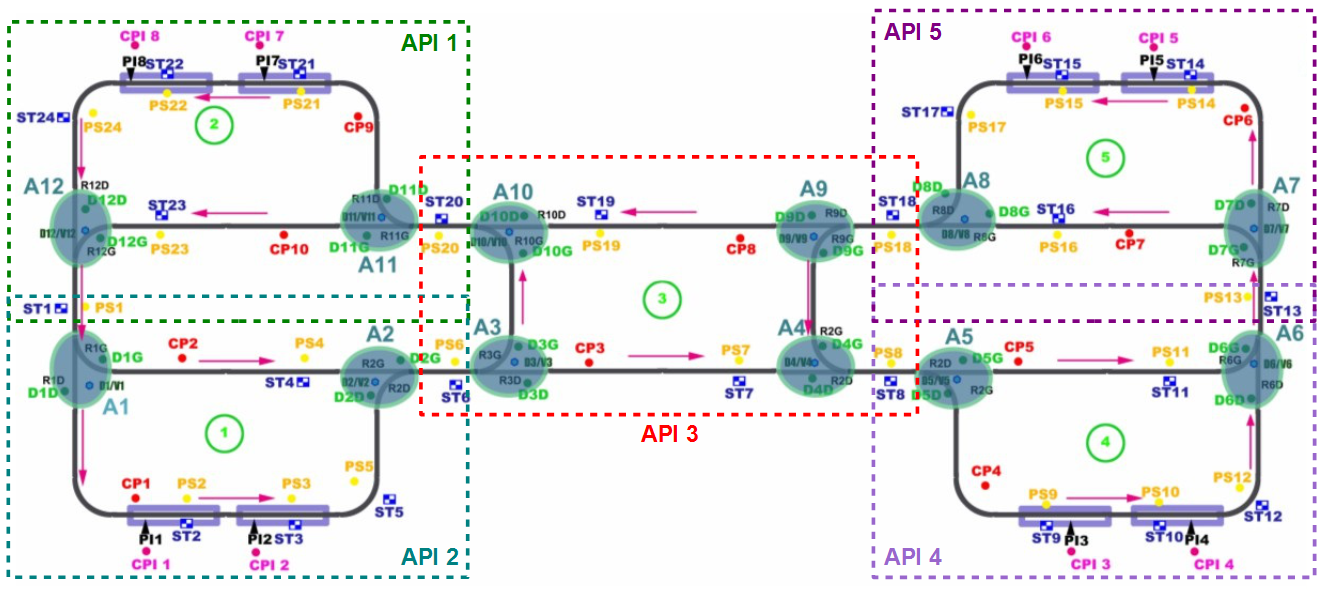
\includegraphics[angle=90,scale=0.72]{Images/maquette.png} 
	     \end{center}
	     \caption{Schéma détaillé de la ligne transitique}
	     \label{Schema_detaille}
\end{figure}

\section{Simulation de la ligne transitique} 

Une simulation de la ligne transitique a été conçue par des étudiant de l'ENSEEIHT à l'aide du logiciel V-REP\footnote{V-REP est une plateforme de simulation pour tout type de robots \hyperref[biblio]{\textbf{[7]}}.}. Cette simulation se comporte comme la ligne MONTRAC$^{\circledR}$, bien qu'elle ne possède pas tous les capteurs et actionneurs (les différences sont détaillés table \ref{tab:capteur_simu}). Elle permet de valider un grand nombre de commandes avant des les tester directement sur la ligne réelle.

\begin{figure}[H]
	     \begin{center}
	     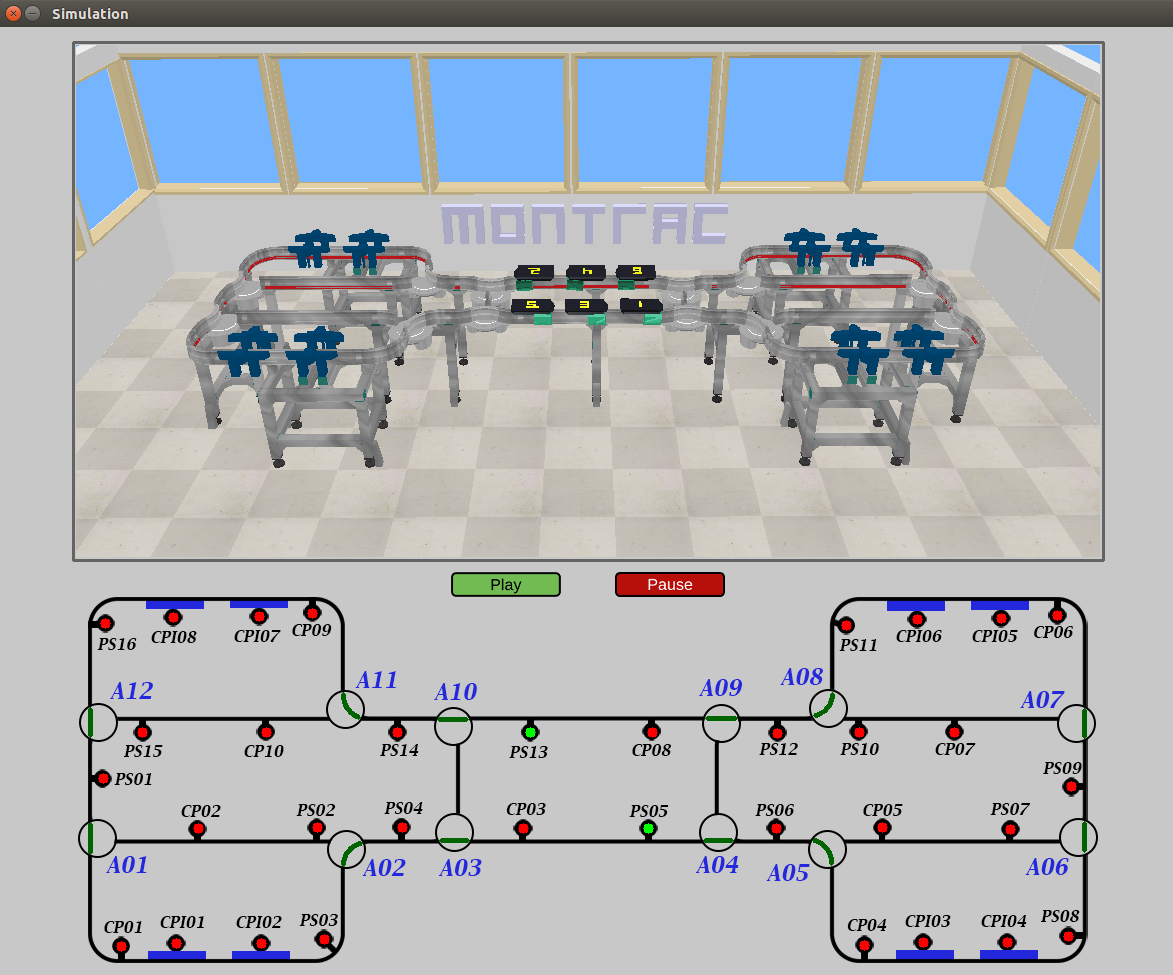
\includegraphics[scale=0.5]{Images/simulation2.png} 
	     \end{center}
	     \caption{Simulation de la ligne transitique}
	     \label{Simulation}
\end{figure}

Pour la conception de la simulation, les étudiants on regroupé les capteurs en catégories : CPI, CP, PS, DG et DD qui correspondent à ceux cités précédemment (table~\ref{tab:capteurs}). Il y a cependant quelques différences pour les capteur PS et CPI comme on peut le voir sur la table \ref{tab:capteur_simu}.


\begin{table}[H]

 	  
\begin{center}
	\begin{tabular}{|c||c|c|c|c|c|c|c|c|c|c|c|c|c|}
	\hline Ligne transitique   &PS1&PS2&PS3&PS4&PS5&PS6&PS7&PS8&PS9&PS10&PS11&PS12&PS13\\
	\hline Simulation   &PS1&CPI1&CPI2&PS2&PS3&PS4&PS5&PS6&CPI3&CPI4&PS7&PS8&PS9\\
	\hline
	\end{tabular} 
	\\[0.7cm]
	\begin{tabular}{|c||c|c|c|c|c|c|c|c|c|c|c|}
	\hline Ligne transitique   &PS14&PS15&PS16&PS17&PS18&PS19&PS20&PS21&PS22&PS23&PS24\\
	\hline Simulation   &CPI5&CPI6&PS10&PS11&PS12&PS13&PS14&CPI7&CPI8&PS15&PS16\\
	\hline
	\end{tabular}       
\end{center}
\caption{\label{tab:capteur_simu}Capteurs de stop de la ligne transitique et de la simulation}
\end{table}

\newpage
Sur la simulation, les capteur CPI ne sont pas les capteurs de position des ergots mais des capteurs de stop aussi. Pour les actionneurs, il y a 5 registres : RD, RG, LOCK, STOP et GO ; RD et RG fonctionnement de la même manière que ceux de la table~\ref{tab:actionneurs} mais LOCK, STOP et GO ont un fonctionnement différent :

\begin{itemize}
\item[ ]
\item[•] LOCKx = $\overline{\text{Vx}}$.Dx
\item[•] STOPx = $\overline{\text{STx}}$
\item[•] GOx = STx
\item[ ]
\end{itemize}




\section{Problématique et solution mise en place}

Comme je l'ai dit précédemment, le but de mon stage était de faire interagir le ligne transitique (ou sa simulation) avec le robot Baxter. Pour cela j'ai utilisé le middleware ROS (Robot Operating System), c'est un ensemble de librairies et d'outils qui permettent de mettre en place toutes sortes d'applications robotiques.\\

Je me suis servi de ce que mon groupe de TER et moi même avions effectué pour établir la communication entre les automates de la ligne transitique et ROS \hyperref[biblio]{\textbf{[5]}}. J'ai alors ajouté la communication de la ligne transitique (ou la simulation) avec le robot Baxter ainsi que sa commande à lui même à l'aide de ROS.\\

Les commandes de la ligne transitique ont été modélisées par des réseaux de Petri (RdP) afin d'utiliser plusieurs navettes en parallèle. Les commandes du robot Baxter ont été modélisé par des machinés à états finis (MEF), une pour chaque bras du robot.\\

La commande ainsi réalisé possède l'architecture figure \ref{schema_solution} que vous pouvez observer ci dessous.

\begin{figure}[H] 
\begin{center}
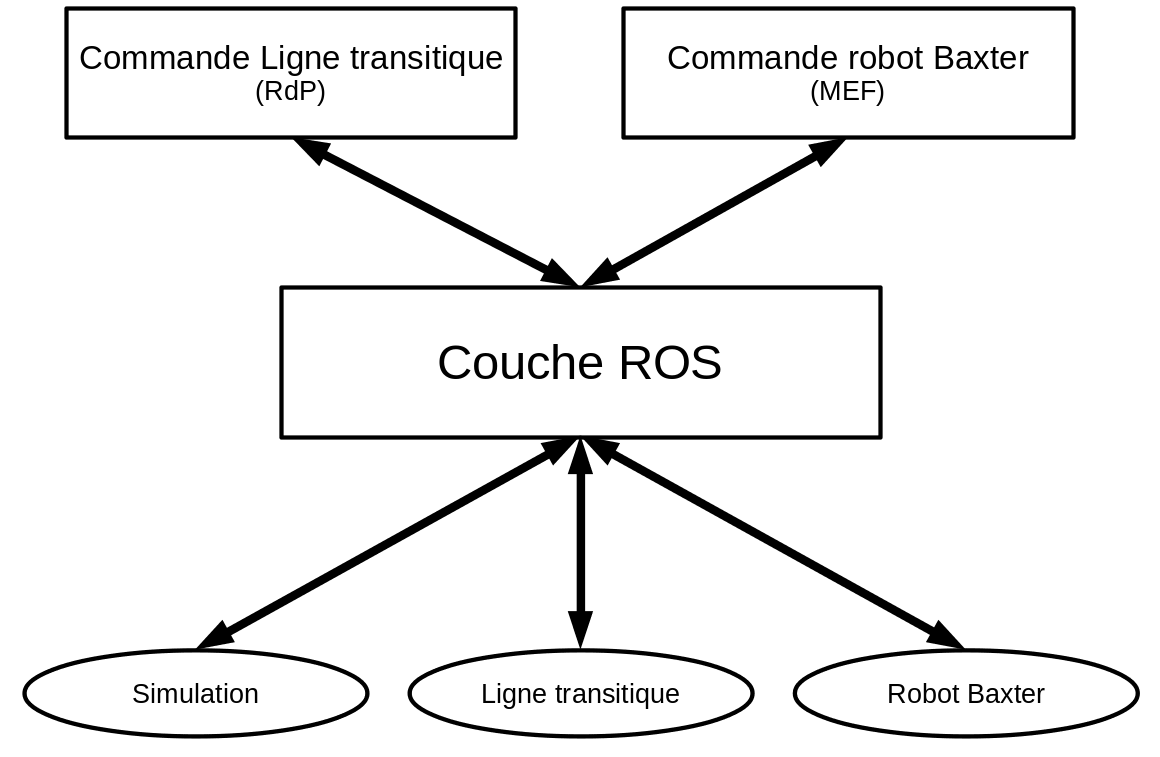
\includegraphics[scale=0.4]{Images/solution.png} 
\end{center}
\caption{Architecture de la solution mise en place}
\label{schema_solution}
\end{figure} 

\newpage
\section{Présentation du middleware ROS}

ROS (Robot Operating System) est une plateforme de développement logiciel qui facilite le développement d'applications robotiques car il permet de créer des pont de communication entre différentes entités de façon très simple. ROS peut être implémenté dans 2 langages : le Python et le C++, nous avons choisi le C++.\\

ROS permet l'échange de messages entre nœuds qui sont stockés dans des répertoires nommés packages. Les nœuds sont des exécutables qui utilisent ROS afin de communiquer avec d'autres nœuds. Pour que les nœuds puissent communiquer entre eux, il faut lancer la plateforme en activant un maître. Les nœuds peuvent échanger alors les informations entre eux soit de manière asynchrone via un topic (sujet) ou de manière synchrone via un service. Chaque nœud ROS évolue en parallèle par rapport aux autres.\\

Le principe des topics est assez simple, il est possible de publier sur un topic ou bien d'y être abonné. Lorsqu'un nœud publie sur un topic, il envoie un message à des instants choisis par le programmeur (à une certaine fréquence ou sous certaines conditions). Lorsqu'un nœud est abonné à un topic, il reçoit tous les messages publiés sur ce topic et pour chaque message reçu, une fonction appelée "Callback" est lancée afin de traiter le message comme on le souhaite. Il est possible de publier sur plusieurs topics et d'être abonné à plusieurs topics à la fois. Pour publier et lire des messages sur un topic, il faut aussi définir les types de messages que l'on souhaite utiliser.\\

Lorsque qu'un nœud utilise un service, il est le client de ce service, il doit alors définir une requête à destination de ce service qui est elle aussi sous forme de message et il recevra ensuite la réponse à sa requête une fois le service appelé.




\begin{figure}[H] 
\begin{center}
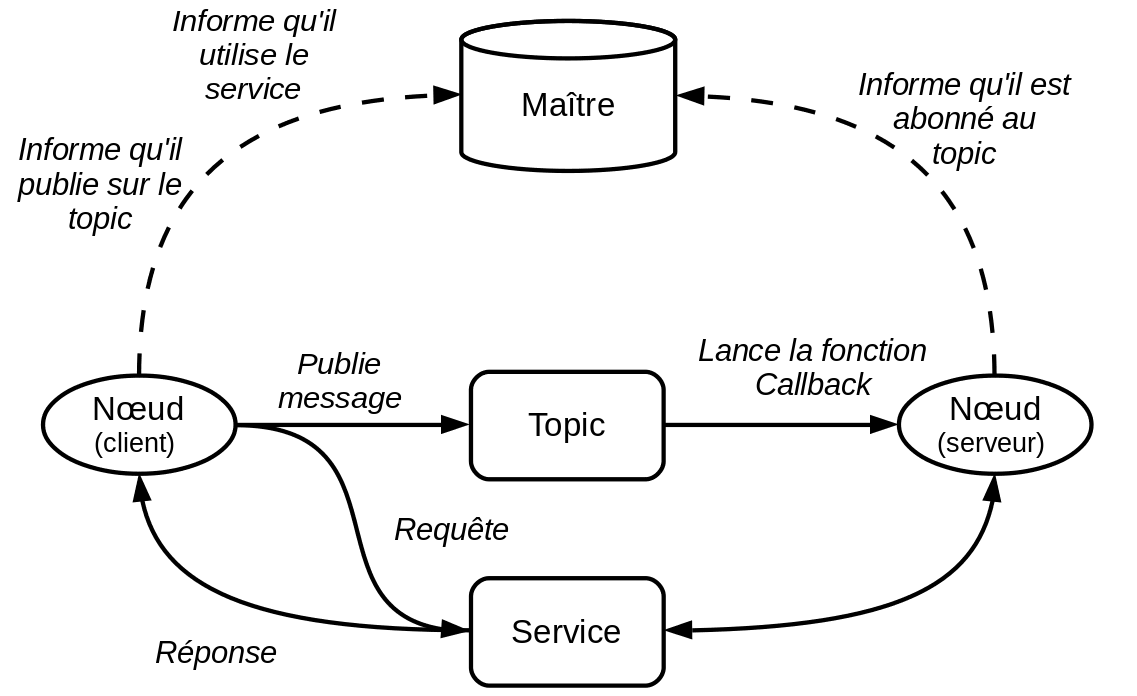
\includegraphics[scale=0.4]{Images/topic.png} 
\end{center}
\caption{Fonctionnement d'un topic sur ROS}
\label{topic}
\end{figure} 

\newpage
\chapter{ROS}



\section{Les topics et services de Baxter}

Afin de communiquer avec Baxter, le robot possède plusieurs topics ROS sur lesquels il publie régulièrement pour envoyer les valeurs de ses capteurs et d'autres auxquels il est abonné pour pouvoir le commander. Je présenterais ici les topics et un service que j'ai utilisés pour la commande de Baxter ainsi que d'autres topics qui peuvent s'avérer utiles.

\subsection{Les topics des états}

\subsubsection{/robot/state}

Ce topic permet de savoir si le robot est activé avant de le commander, il utilise des messages de type "baxter$\_$core$\_$msgs/AssemblyState.msg" :\\

\begin{tabular}{ll}
bool enabled & \\
bool stopped & \\
bool error & \\
uint8 estop$\_$button & \\
uint8 estop$\_$source & \\
\end{tabular}



\subsubsection{/robot/joint$\_$states}

Ce topic permet de connaitre l'état de chacun des angles du robot (nom, position, vitesse et effort), il utilise des messages de type "sensor$\_$msgs/JointState.msg" :\\

\begin{tabular}{l}
std$\_$msgs/Header header\\
string[] name\\
float64[] position\\
float64[] velocity\\
float64[] effort\\
\end{tabular}

\subsubsection{/robot/limb/left/endpoint$\_$state et /robot/limb/right/endpoint$\_$state}

Ces topics permettent de connaître la position des extrémités des bras en cordonnées cartésiennes (pose.position), ainsi que leur orientation en quaternions (pose.quaternions) et les efforts qui sont exercés à ces extrémités (twist et wrench). Les messages sont de type "baxter$\_$core$\_$msgs/EndpointState.msg" :\\

\begin{tabular}{l}
geometry$\_$msgs/Pose   pose\\
geometry$\_$msgs/Twist  twist\\
geometry$\_$msgs/Wrench wrench\\
\end{tabular}\\

avec "geometry$\_$msgs/Pose.msg" :\\

\begin{tabular}{l}
geometry$\_$msgs/Point position\\
geometry$\_$msgs/Quaternion orientation\\
\end{tabular}

\subsubsection{/robot/end$\_$effector/left$\_$gripper/state et /robot/end$\_$effector/right$\_$gripper/state}

Ces topics permettent de connaître l'état de la pince du bras gauche ou droit, ils utilisent les messages de type "baxter$\_$core$\_$msgs/EndEffectorState" :\\

\begin{tabular}{l}
time timestamp\\
uint32 id \\
uint8 enabled\\
uint8 calibrated\\
uint8 ready\\
uint8 moving\\
uint8 gripping\\
uint8 missed\\
uint8 error\\
uint8 reverse\\
float32 position\\
float32 force\\
string state\\
string command\\
string command$\_$sender\\
uint32 command$\_$sequence\\
\end{tabular}\\

\subsection{Les topics de commande}

\subsubsection{/robot/set$\_$super$\_$enable}

Ce topic permet d'activer le robot afin de le commander, il utilise des message de type "std$\_$msgs/Bool.msg" :\\

\begin{tabular}{l}
bool data\\
\end{tabular}

\subsubsection{/robot/limb/left/joint$\_$command et /robot/limb/right/joint$\_$command}

Ces topics permettent de commander les bras du robot suivant les modes décrit dans \ref{section_lerobotbaxter}, ils utilisent les messages de type "baxter$\_$core$\_$msgs/JointCommand.msg" :\\

\begin{tabular}{l}
int32 mode\\
float64[] command\\
string[] names\\
\end{tabular}\\

\subsubsection{/robot/end$\_$effector/left$\_$gripper/command et /robot/end$\_$effector/right$\_$gripper/command}

Ces topics permettent de commander les pinces gauche ou droite, ils utilisent les messages de type "baxter$\_$co-
re$\_$msgs/EndEffectorCommand" : \\

\begin{tabular}{l}
uint32 id\\      
string command \\ 
string args  \\   
string sender \\  
uint32 sequence\\
\end{tabular}\\

\subsection{Le service Inverse Kinematics}

\newpage
\section{Les topics de communication entre Baxter et la ligne transitique}

Afin d'établir la communication entre le robot Baxter et la ligne transitiquen j'ai défini des topics supplémentaires qui utilisent tous des messages de type "std$\_$msgs/Bool.msg" :

\begin{itemize}
\item[ ] 
\item[•] \textbf{/pont$\_$BaxterLigneTransitique/<left/right>$\_$arm/attente$\_$prise} : Ce topic permet au robot Baxter d'indiquer à la ligne transitique qu'il est en attente d'une prise pour le bras gauche ou droit.
\item[ ]
\item[•] \textbf{/pont$\_$BaxterLigneTransitique/<left/right>$\_$arm/prise$\_$demandee} : Ce topic permet à la ligne transitique de demander un prise au robot avec le bras gauche ou droit.
\item[ ]
\item[•] \textbf{/pont$\_$BaxterLigneTransitique/<left/right>$\_$arm/prise$\_$effectuee} : Ce topic permet au robot de notifier la ligne qu'une prise avec le bras gauche ou droit a été effectuée.
\item[ ]
\end{itemize}



\section{Le noeud Commande$\_$Baxter}

\subsection{La classe Baxter}

\subsubsection{Attributs}

\subsubsection{Méthodes}


\subsection{Les classes Baxter$\_$left$\_$arm et Baxter$\_$right$\_$arm}

\subsubsection{Attributs}

\subsubsection{Méthodes}


\section{Le noeud Commande}

\subsection{Les classes Capteurs et Actionneurs}

Rappel

\subsection{La classe Communication$\_$Baxter}

\subsubsection{Attributs}

\subsubsection{Méthodes}







\newpage
\chapter{Synthèse de commande}

\subsection{Commande du robot seul}

\begin{figure}[H] 
\begin{center}
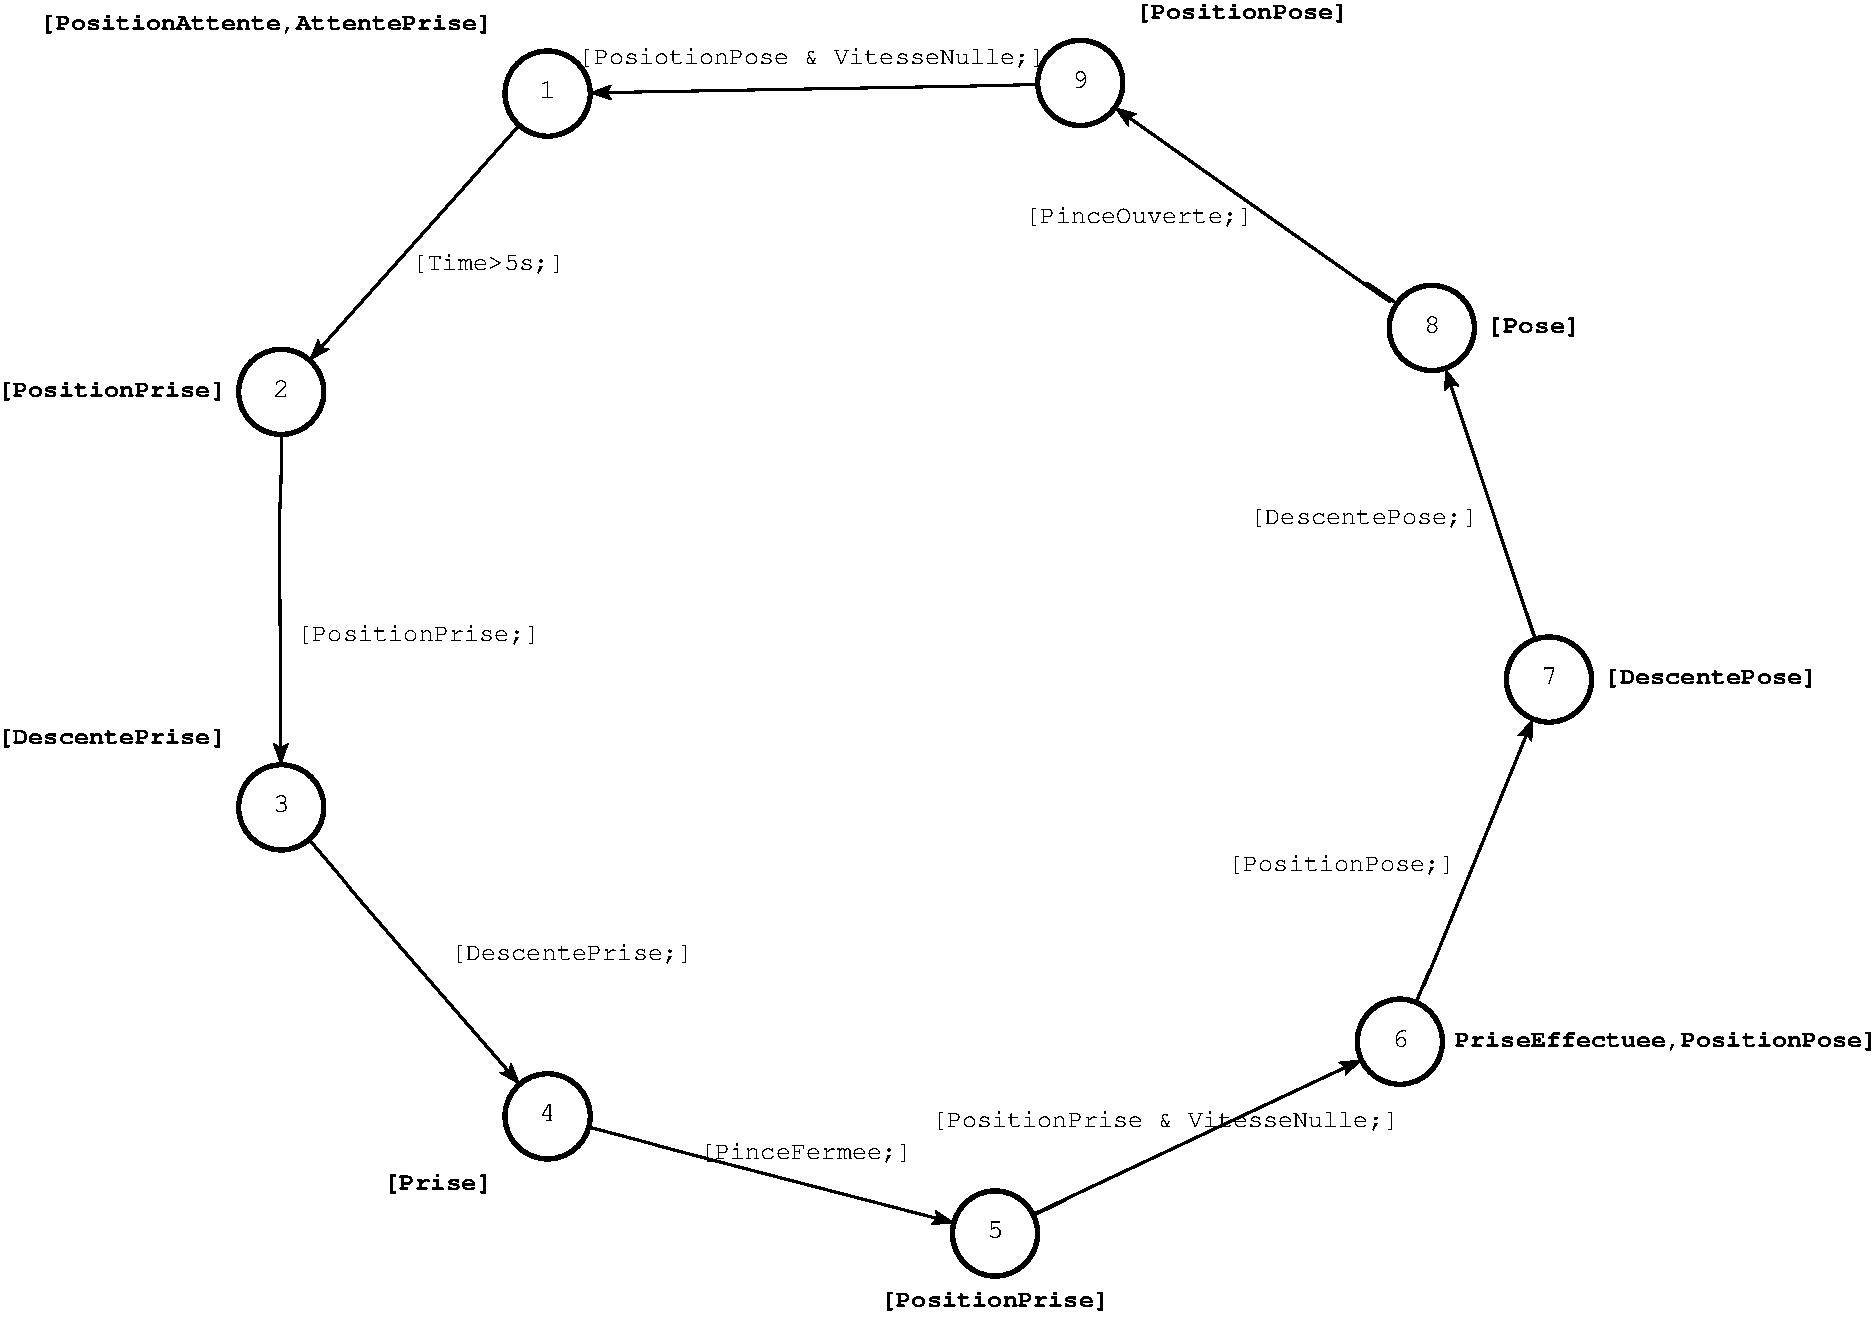
\includegraphics[scale=0.5]{Images/main_commande_1_bras.pdf} 
\end{center}
\caption{Machine à états finis de la commande d'un bras du robot Baxter}
\label{main_commande_1_bras}
\end{figure} 

\subsection{Commande de la ligne transitique MONTRAC en intération avec le robot Baxter}

\begin{figure}[H] 
\begin{center}
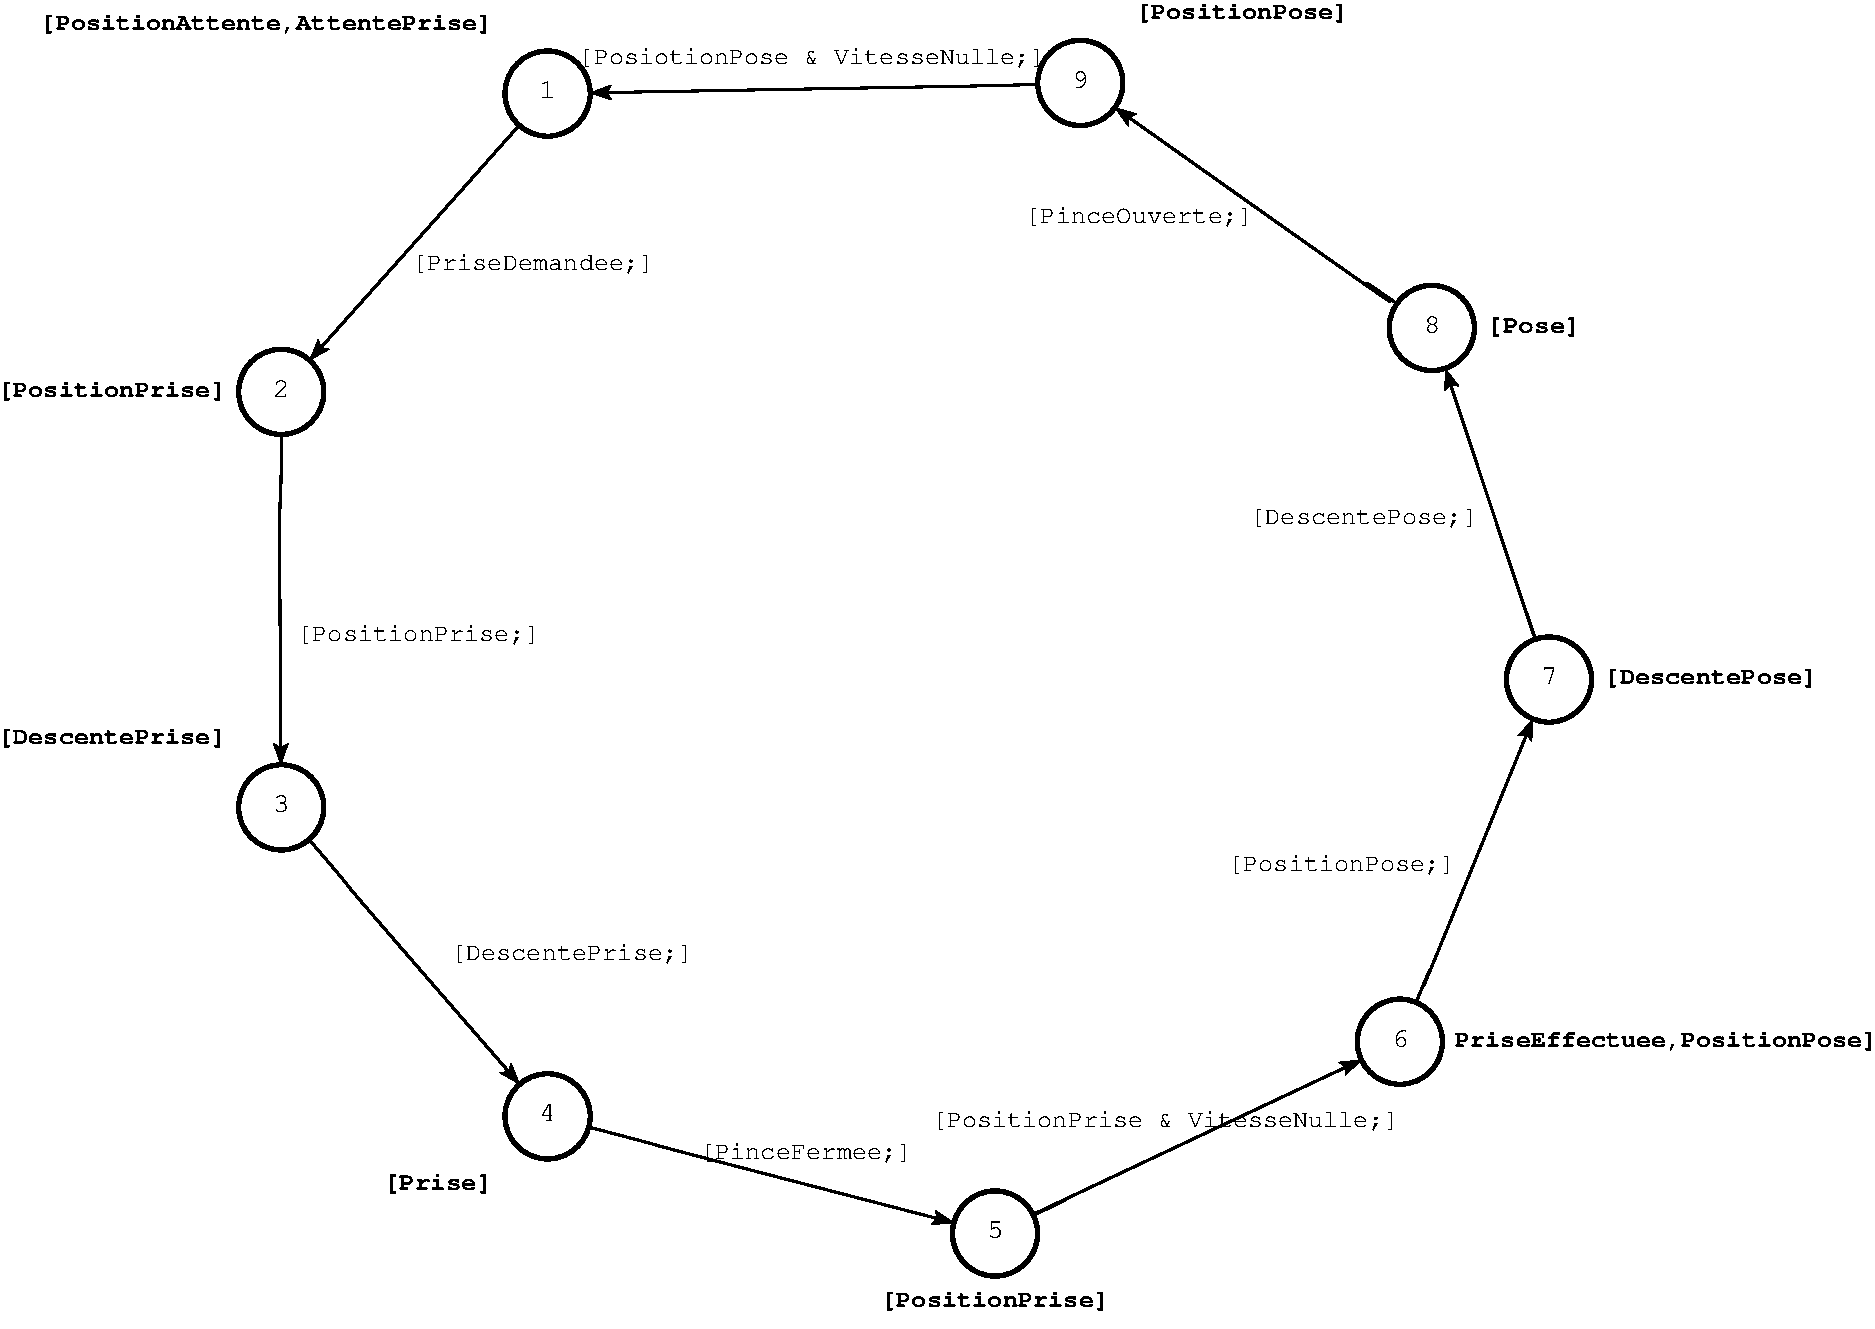
\includegraphics[scale=0.5]{Images/main_commande_bras_GD.pdf} 
\end{center}
\caption{Machine à états finis de la commande de chaqu'un des deux bras en interaction avec la ligne transitique}
\label{main_commande_bras_GD}
\end{figure}

\subsubsection{Commande de la ligne transitique en interaction avec un des bras manipulateurs}

 

\begin{figure}[H] 
\begin{center}
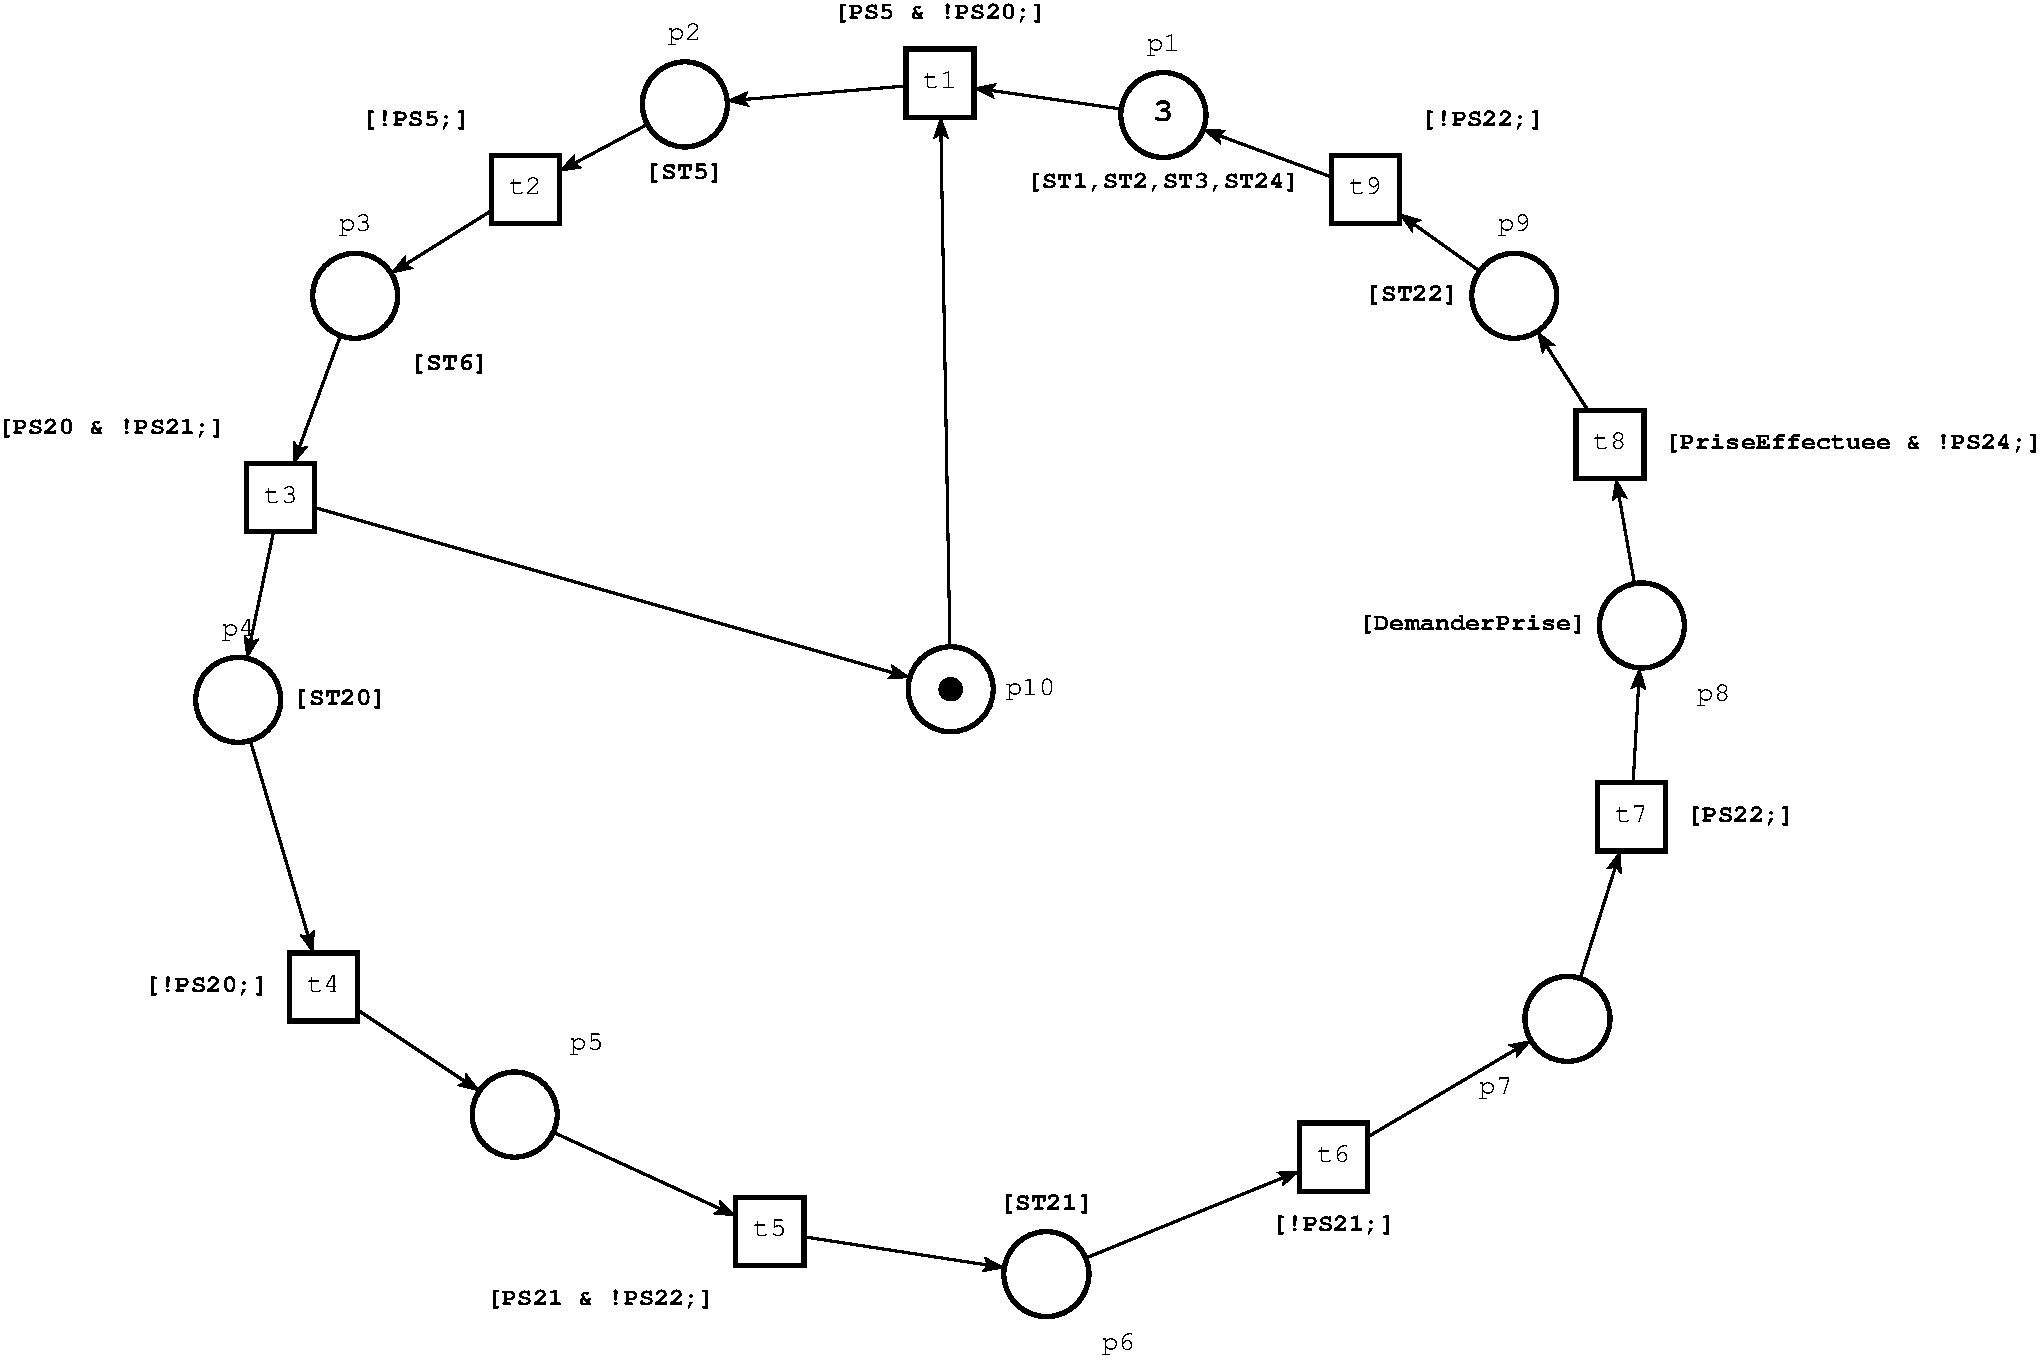
\includegraphics[scale=0.5]{Images/main_commande_baxter_1_bras_ligne_transitique.pdf} 
\end{center}
\caption{Réseau de Petri de la commande de la ligne transitique en interaction avec un bras du robot Baxter}
\label{main_commande_baxter_1_bras_ligne_transitique}
\end{figure}

\subsubsection{Commande de la ligne transitique en interaction avec les deux bras manipulateurs}


\begin{figure}[H] 
\begin{center}
\Rotatebox{90}{
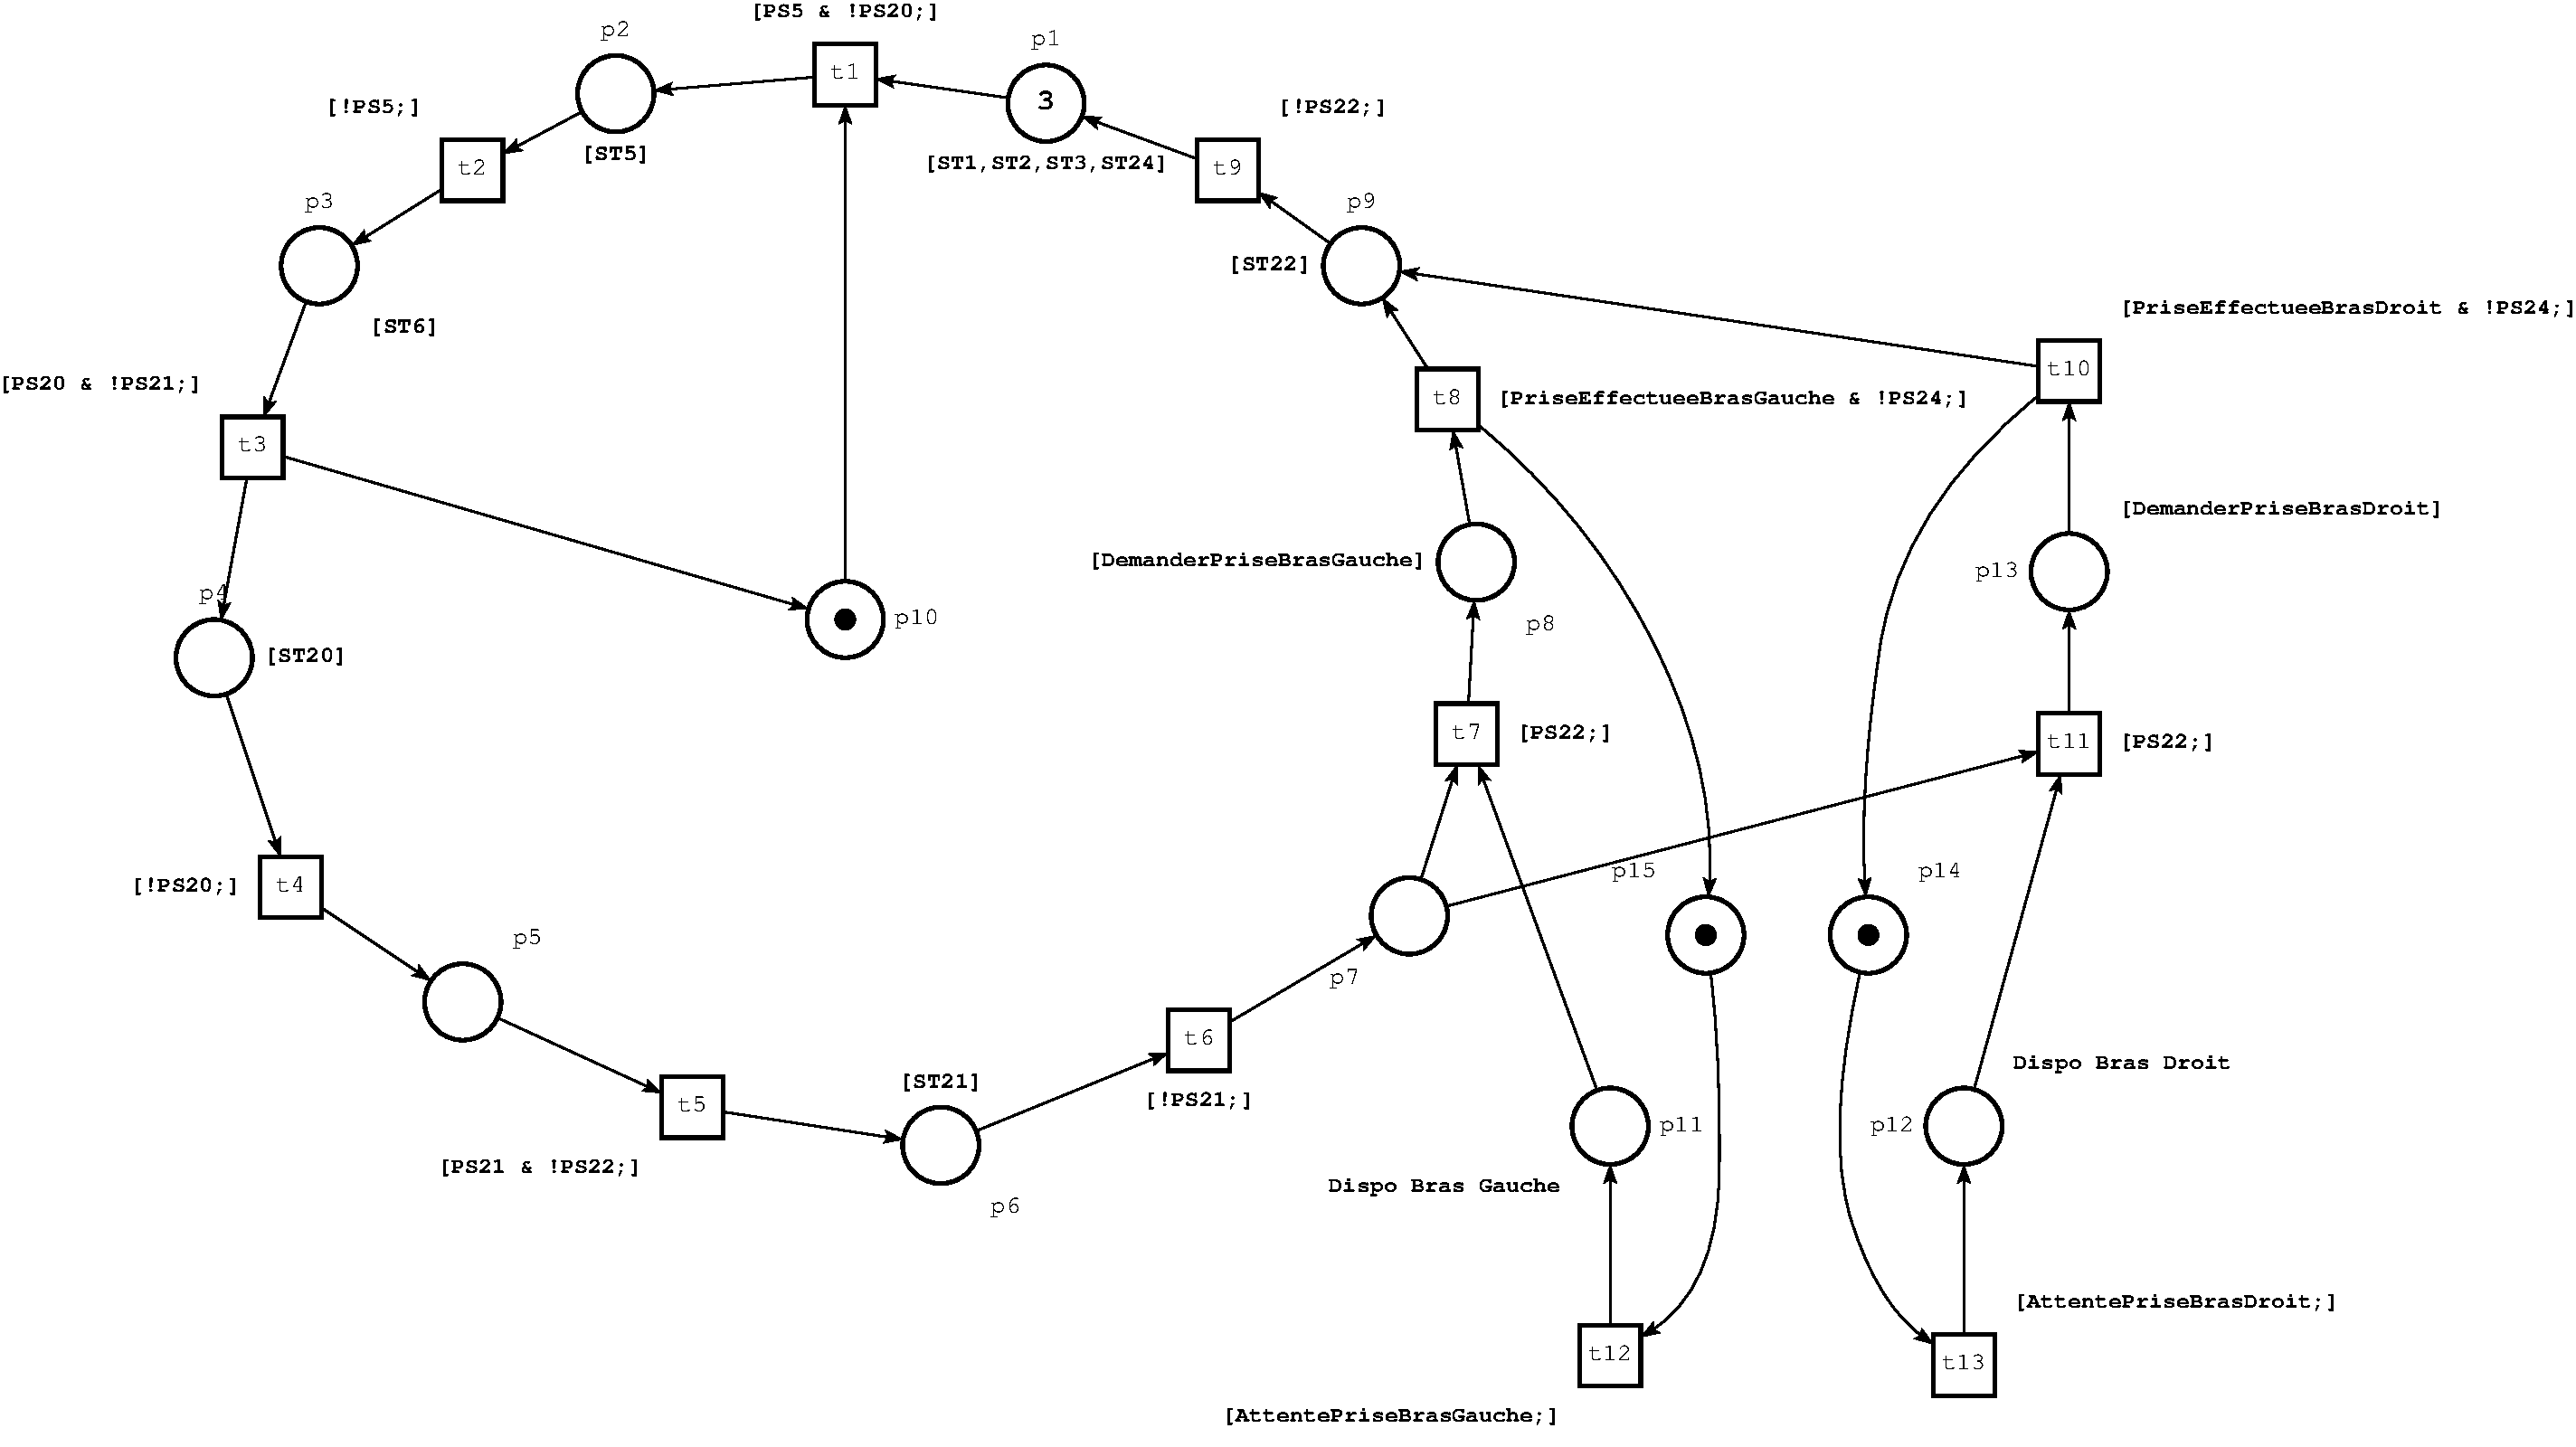
\includegraphics[scale=0.45]{Images/main_commande_baxter_2_bras_ligne_transitique.pdf} 
}
\end{center}
\caption{Réseau de Petri de la commande de la ligne transitique en interaction avec les deux bras du robot Baxter}
\label{main_commande_baxter_2_bras_ligne_transitique}
\end{figure}


\newpage
\addcontentsline{toc}{section}{Conclusion}
\chapter*{Conclusion}


\newpage
\addcontentsline{toc}{section}{Bibliographie}
\chapter*{Bibliographie}\label{biblio}



\begin{itemize}
\item[ \textbf{[1]}] ABIVEN Cédric, CARDONE Grégoire, GAO Shengheng. \textit{Commande d'une ligne transitique MONTRAC}. Rapport de TER, Master 1 Électronique Électrotechnique Automatique, Ingénierie des Sytèmes Temps-Réel. Toulouse : Université Paul Sabatier, 2015.
\item[ ]
\item[ \textbf{[2]} ] ANTONIUTTI Emilie, BERTIN Thibault, DEMMER Simon, LE BIHAN Clément. \textit{Commande et Simulation d'un réseau de transport d'un système de production}. Rapport de Projet Long, GEA CDISC. Toulouse : ENSEEIHT, 2016.\\
Disponible sur <\verb!https://github.com/ClementLeBihan/CelluleFlexible/blob/master/Livrables/R!\\
\verb!apport_Projet_Long!> (Consulté le 26.05.2016)
\item[ ]
\item[ \textbf{[3]} ] ANTONIUTTI Emilie, BERTIN Thibault, DEMMER Simon, LE BIHAN Clément. \textit{Simulation de la ligne transitique MONTRAC}. Code source (GIT). Toulouse : ENSEEIHT, 2016.\\
Disponible sur <\verb!https://github.com/ClementLeBihan/CelluleFlexible!> (Consulté le 26.05.2016)
\item[ ]
\item[ \textbf{[4]} ] GORRY POLLET Alexandra. \textit{Commande d’une cellule flexible de production robotisée}. Rapport de stage, IUT Génie Électrique et Informatique Industrielle. Toulouse : Université Paul Sabatier, 2015.
\item[ ]
\item[ \textbf{[5]}] DATO Bruno, ELGOURAIN Abdellah, SHULGA Evgeny. \textit{Commande d'une ligne transitique MONTRAC}. Rapport de TER, Master 1 Électronique Électrotechnique Automatique, Ingénierie des Sytèmes Temps-Réel. Toulouse : Université Paul Sabatier, 2016.
\item[ ]
\item[ \textbf{[6]} ] AIP-PRIMECA. \textit{Pôle AIP-PRIMECA Toulouse}.\\
Disponible sur <\verb!http://aip-primeca.ups-tlse.fr/!> (Consulté le 26.05.2016)
\item[ ]
\item[ \textbf{[7]} ] Robot Operating System. \textit{ROS}.\\
Disponible sur <\verb!http://www.ros.org/!> (Consulté le 26.05.2016)
\item[ ]
\item[ \textbf{[8]} ] V-REP. \textit{v-rep virtual robot experimentation platform}.\\
Disponible sur <\verb!http://www.coppeliarobotics.com/!> (Consulté le 26.05.2016)
\item[ ]
\end{itemize}

\end{document}



